\documentclass[11pt]{article}
\usepackage{graphicx} % Required for inserting images
\usepackage{amsmath}
\usepackage{listings}
\graphicspath{ {./lab1} }

\begin{document}

\begin{titlepage}
   \begin{center}
       \vspace*{1cm}
       \textbf{\Huge Numerical Methods} \\
        \vspace{2.0cm}
        \huge{Laboratory no. 1}
         \vspace{.7cm}
       \huge{\\ \today}
        \vspace{3.0cm}
         \vspace{0.4cm}
        Krzysztof Watras\\
        \vspace{2 cm}   
       \small{Computer Science} \\  
       \vspace{0.2cm}       
       \small{Warsaw University of Technology} 
       \date{\today}
   \end{center}
\end{titlepage} 

\begin{center}
\textbf{\Large  Documentation of laboratory work results }\\ 
\end{center}

\section*{Task 1}
Given a function $$y = \frac{\cos(x)}{x^3} - x^2$$ we want to calculate it's T(x) coefficient.
We will use the property 
$$\sigma [\tilde{v}^k] = T^k \cdot \sigma[\tilde{x}^{k-1}] + \nu^k$$
In our function we use:
\begin{align*}
    v_1 &= \cos(x) \\ 
    v_2 &= x^3 \\ 
    v_4 &= \frac{v_1}{v_2} \\ 
    v_4 &= x^2 \\ 
    y &= v_4 - v_4 \\ 
\end{align*}
Therefore we obtain:
\begin{align*}
    \tilde{v_1} &= \cos(x(1+\epsilon_1)) \\ 
    \tilde{v_2} &= (x(1+\epsilon))^3 = x^3 (1+3\epsilon_2) \\ 
    \tilde{v_3} &= \frac{\tilde{v_1}}{\tilde{v_2}} \\ 
    \tilde{v_4} &= (x(1+\epsilon))^2 = x^2 (1+2\epsilon_4) \\
    \tilde{y} &= \tilde{v_3} - \tilde{v_4} \\ 
\end{align*}
Let us focus on $\tilde{ v_1 }$:
$$ \cos(x(1+\epsilon)) = \cos(x+x\epsilon) = \cos(x)\cos(x\epsilon) - \sin(x)\sin(x\epsilon) $$
Now we need to use property of trigonometric functions: 
$$For\ \alpha \rightarrow 0, \sin(\alpha) \approx \alpha , \cos(\alpha) \approx 1-\frac{ \alpha^2 }{ 2 }$$
Using those properties:
\begin{align*}
    \cos(x(1+\epsilon)) &= \cos(x)\cos(x\epsilon) - \sin(x)\sin(x\epsilon)\\
    &= \cos(x)(1-\frac{(x\epsilon)^2}{2}) - \sin(x)x\epsilon \\
    &= \cos(x) - \sin(x)x\epsilon\\
    &= \cos(x)\cdot (1-\tan(x)x\epsilon)
\end{align*}
Now solve $v_3$:
\begin{align*}
    \tilde{v_3} &= \displaystyle\frac{\cos(x) \cdot (1 - x\tan(x) \epsilon_1)}{x^3 (1+3\epsilon_2)}\\
    &= \frac{\cos(x)}{x^3} (1 - x\tan(x) \epsilon_1)\cdot (1+3\epsilon_2)^{-1}\\
    &= \frac{\cos(x)}{x^3} (1 - x\tan(x) \epsilon_1)\cdot (1-3\epsilon_2)\\
    &= \frac{\cos(x)}{x^3} (1 - x\tan(x) \epsilon_1 - 3\epsilon_2)\\
\end{align*}
Finally, we get:
\begin{align*}
\tilde{y}&=\frac{\cos(x)}{x^3}(1 - x\tan(x) \epsilon_1 - 3\epsilon_2)-x^2(1+2\epsilon_4)\\
    &=\frac{\cos(x)}{x^3}-\frac{\cos(x)}{x^3}(x\tan(x) \epsilon_1 + 3\epsilon_2)-x^2-2x^2\epsilon_4 \\
    &=y-\frac{\cos(x)}{x^3}(x\tan(x) \epsilon_1 + 3\epsilon_2)-2x^2\epsilon_4\\
    &=y(1 + (-\frac{\cos(x)}{x^3}(x\tan(x) \epsilon_1 + 3\epsilon_2)-2x^2\epsilon_4)\frac1y)\\
    &=y(1 + (-\frac{\sin(x)}{x^2}\epsilon_1 - 3\frac{\cos(x)}{x^3}\epsilon_2 - 2x^2\epsilon_4)\frac1y)\\
\end{align*}
Therefore, 
$$T(x) = \displaystyle\frac{
\left|-\frac{\sin(x)}{x^2}\right| +
\left|- 3\frac{\cos(x)}{x^3}\right| +
\left|-2x^2\right|
}
{\frac{\cos(x)}{x^3} - x^2}$$

This yields results simmilar to the ones we got via calculating the error numerically.
Function $$T(x) = \frac{1}{\epsilon_{sim}}\left| \displaystyle\frac{y(\tilde{x}) - y(x)}{y(x)} \right|$$
Does not differ significantly from the one we got from analitical solution.\\
Graph that visualises both:\\
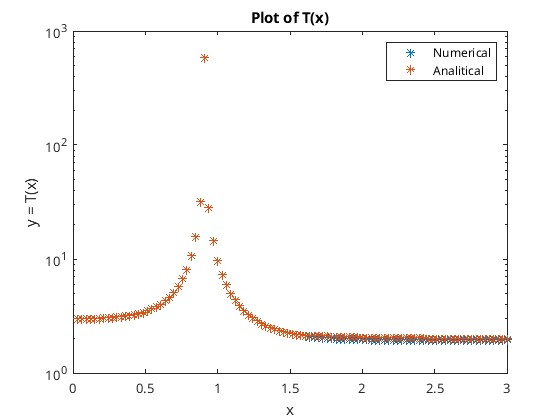
\includegraphics[width=\textwidth]{Task1.jpg}

\pagebreak
Code I used to obtain such graph:
\begin{lstlisting}[language=matlab]
% clear previous experiment results
clc, clearvars, close all

% define domain and function
x = linspace(0,3,100);
y = @(x) cos(x)./x.^3 - x.^2;
% define erronous domain
esim = 1.0e-8;
x_eps = x.*(1+esim);
% calculate true y and epsilon y
ydot = y(x);
yeps = y(x_eps);
% calculate T numerically
numerator = yeps - ydot;
abs_error = abs(numerator ./ ydot);
tx = 1/esim * abs_error;

% calculate T analiticaly (formula calculated in the report)
T1 = -sin(x)./(x.^2);
T2 = -3*cos(x)./(x.^3);
T3 = 2*x.^2;

Tn = (abs(T1) + abs(T2) + abs(T3));
tx_analitical = Tn./abs(ydot);

% plot results to validate both methods result in simmilar results
semilogy(x,tx, '*');
hold on 
semilogy(x,tx_analitical, '*');
title("Plot of T(x)"), xlabel("x"), ylabel("y = T(x)"),
legend("Numerical", "Analitical")
\end{lstlisting}

\pagebreak
\section{Task 2}
\end{document}

